%
%
%
\subsection{Beam-variation hardened calibration results {\color{blue} Laurence $\rightarrow$ Juan}}
%\label{se:valid_photocorr_cal}

%  PHOTOCORR DEMO
%_____________________________________________________________________
\subsubsection{The demonstration case}
\addparag{ demonstration case}

We assess the beam-variation hardened calibration for the
demonstration case, as discussed in Sect.~\ref{se:cal_democase}.
The upper panels of Fig.~\ref{fig:mwc349_flux_obstau_photocorr} shows
the measured-to-expected flux density
ratio of MWC349 using the demaonstration case calibration, and
Table~\ref{tab:photocorr_demo_calib_result_mwc349} gathers the
calibration results. 

\begin{figure}[ht!]
  \begin{center}
%    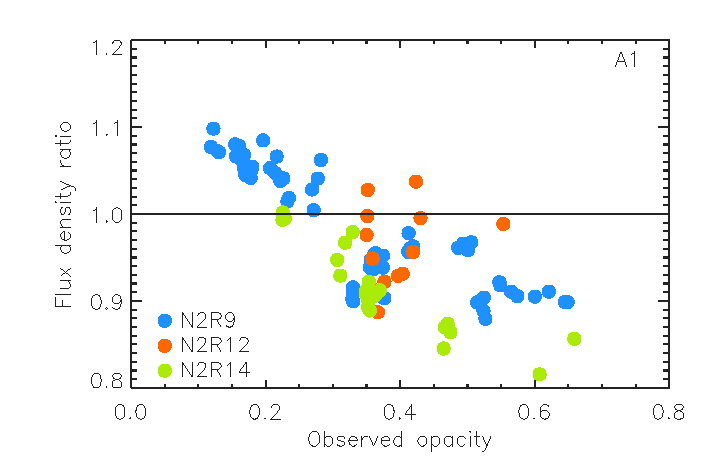
\includegraphics[clip=true,width=0.47\textwidth]{Figures/Calibration/Photocorr/plot_flux_density_ratio_MWC349_obstau_secondary_photocorr_demo_a1.pdf}
%    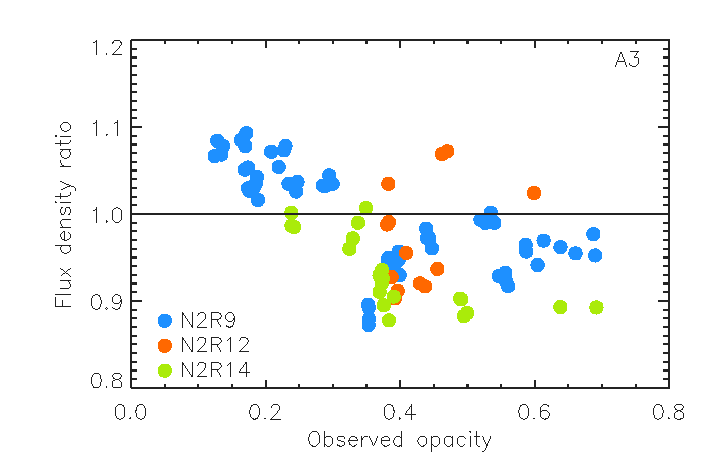
\includegraphics[clip=true,width=0.47\textwidth]{Figures/Calibration/Photocorr/plot_flux_density_ratio_MWC349_obstau_secondary_photocorr_demo_a3.pdf}
    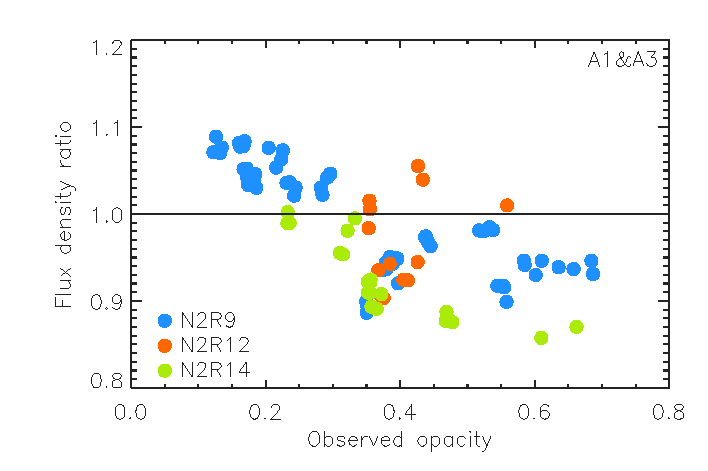
\includegraphics[clip=true,width=0.47\textwidth]{Figures/Calibration/Photocorr/plot_flux_density_ratio_MWC349_obstau_secondary_photocorr_demo_1mm.pdf}
    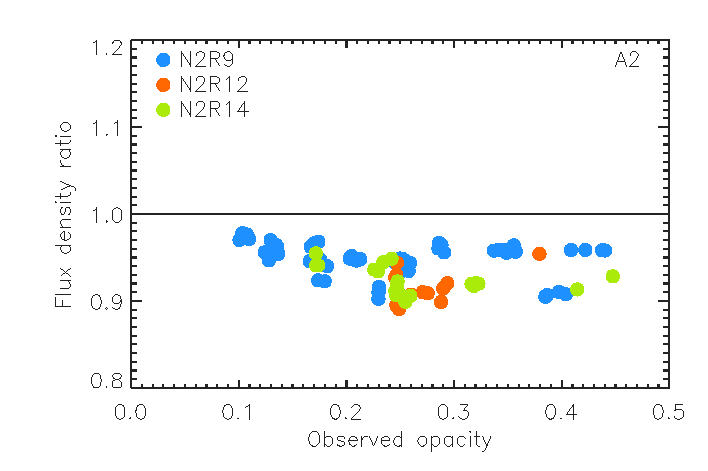
\includegraphics[clip=true,width=0.47\textwidth]{Figures/Calibration/Photocorr/plot_flux_density_ratio_MWC349_obstau_secondary_photocorr_demo_a2.pdf}
    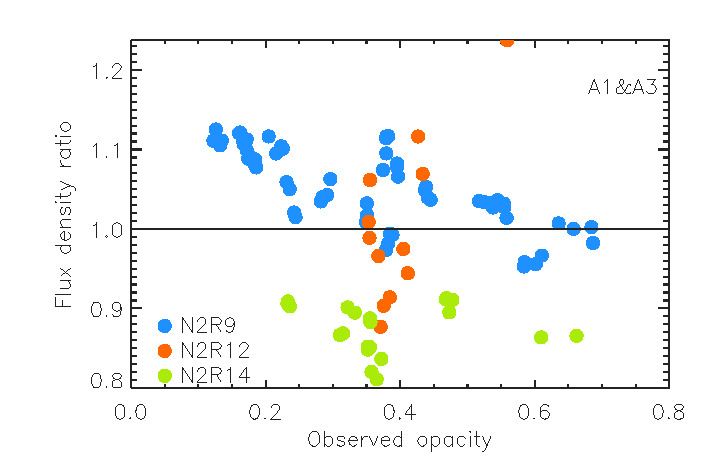
\includegraphics[clip=true,width=0.47\textwidth]{Figures/Calibration/Photocorr/plot_flux_density_ratio_MWC349_obstau_secondary_photocorr_pointing_1mm.pdf}
    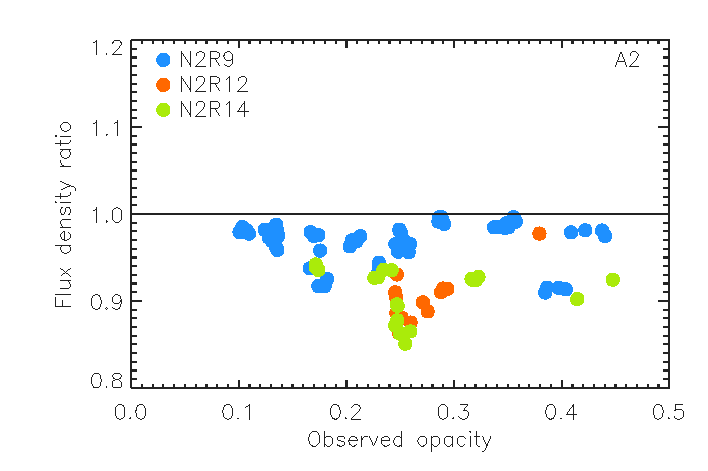
\includegraphics[clip=true,width=0.47\textwidth]{Figures/Calibration/Photocorr/plot_flux_density_ratio_MWC349_obstau_secondary_photocorr_pointing_a2.pdf}
    
    \caption[Validation of the beam-variation hardened calibration
      using MWC349 flux density]{Validation
      of the beam-variation hardened calibration for the demonstration
      case (top) and for the practical case (bottom).
      Datapoints show the measured-to-modeled flux density ratio for the
      secondary calibrator MWC349 as a fonction
      of the measured observed opacity for the 1mm array combination
      (left) and for array 2 (right). The color coding is the same as
      in Fig.~\ref{fig:mwc349_flux_obstau}.
    }
    \label{fig:mwc349_flux_obstau_photocorr}
  \end{center}
\end{figure}



\begin{table}[th]
\begin{center}
\begin{tabular}{|c|c|cccc|}
\hline
Runs & Arrays & $\#$Total scans   & $\#$Selected scans & Flux density bias  & Relative error \\ 
\hline\hline
 N2R9   & A1        & 64                 &  64         & 0.98               &  6.8    \\ 
        & A3        &                    &             & 0.99               &  6.0     \\ 
        & A1$\&$A3  &                    &             & 0.99               &  6.2    \\ 
        & A2        &                    &             & 0.95               &  1.9    \\ 
 \hline
 N2R12  & A1        & 13                 &  13         & 0.96               &  4.8    \\ 
        & A3        &                    &             & 0.97               &  6.2    \\ 
        & A1$\&$A3  &                    &             & 0.97               &  5.4    \\ 
        & A2        &                    &             & 0.92               &  2.1     \\
 \hline
 N2R14  & A1        & 21                 &  21         & 0.91               &  5.7  \\ 
        & A3        &                    &             & 0.93               &  4.6   \\ 
        & A1$\&$A3  &                    &             & 0.92               &  5.0   \\ 
        & A2        &                    &             & 0.92               &  1.7   \\
 \hline
combined & A1        &  98                & 98         &  0.97              &  7.0  \\ 
         & A3        &                    &            &  0.98              &  6.3  \\ 
         & A1$\&$A3  &                    &            &  0.97              &  6.4   \\ 
         & A2        &                    &            &  0.94              &  2.4  \\
\hline\hline
\end{tabular}
\caption[Beam-variation hardened calibration results using MWC349: the
demonstration case]{Beam-variation hardened calibration results using
  MWC349 photometry: the demonstration case. For the observation runs or combination of runs indicated in the first column, we report the total number of observation scans in the third column, the number of scan after the baseline selection in the fourth column, the flux density biases in the fifth, which correspond to the average measured-to-expected flux density ratios, and the relative errors given in percent in the last column, which are the $1\sigma$ errors with respect to the mean flux densities.}
\label{tab:photocorr_demo_calib_result_mwc349}
\end{center}
\end{table}


The flux density stability against the estimated beam size is also
checked using other secondary calibrators in the upper panels of
Fig.~\ref{fig:photocorr_secondcalib_flux_1_2_mm}.


\begin{figure}[ht!]
  \begin{center}
    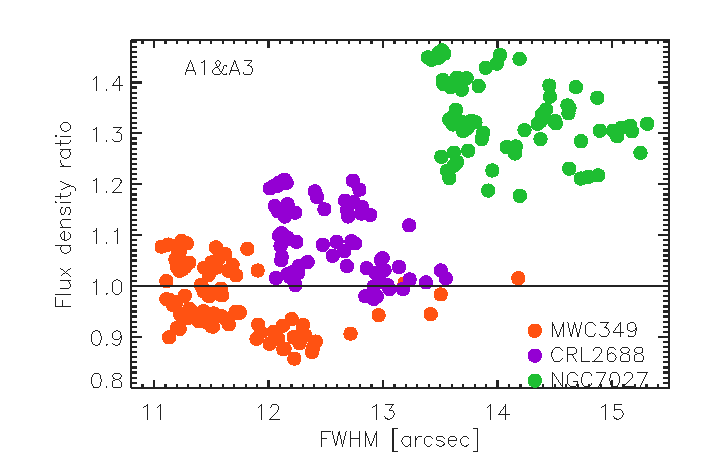
\includegraphics[clip=true,width=0.47\textwidth]{Figures/Calibration/Photocorr/plot_flux_density_ratio_3sources_FWHM_secondary_photocorr_demo_1mm.pdf}
    \includegraphics[clip=true,width=0.47\textwidth]{Figures/Calibration/Photocorr/plot_flux_density_ratio_3sources_FWHM_secondary_photocorr_demo_A2.pdf}
   % 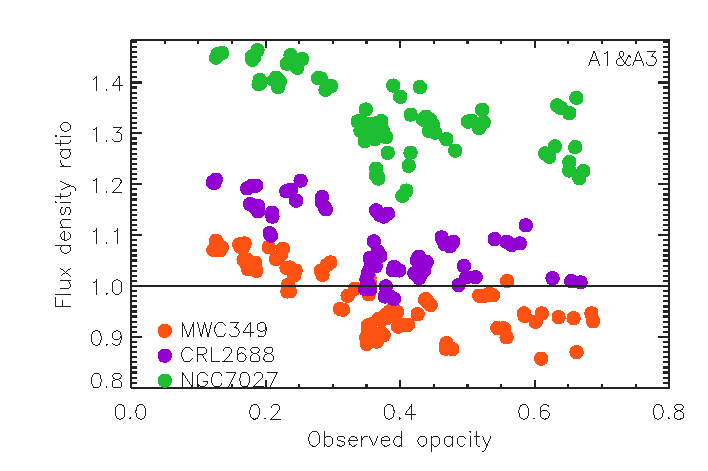
\includegraphics[clip=true,width=0.47\textwidth]{Figures/Calibration/Photocorr/plot_flux_density_ratio_3sources_obstau_secondary_photocorr_demo_1mm.pdf}
    %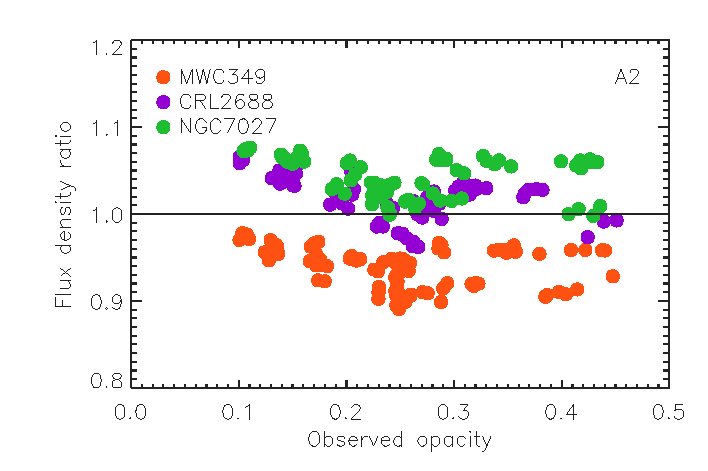
\includegraphics[clip=true,width=0.47\textwidth]{Figures/Calibration/Photocorr/plot_flux_density_ratio_3sources_obstau_secondary_photocorr_demo_a2.pdf}
    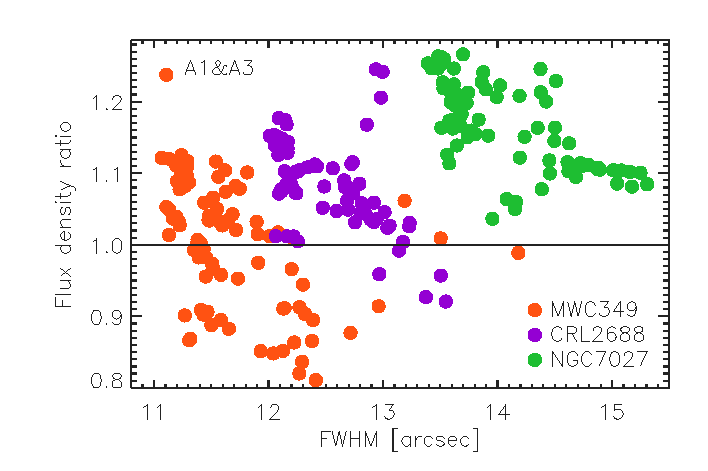
\includegraphics[clip=true,width=0.47\textwidth]{Figures/Calibration/Photocorr/plot_flux_density_ratio_3sources_FWHM_secondary_photocorr_pointing_1mm.pdf}
    \includegraphics[clip=true,width=0.47\textwidth]{Figures/Calibration/Photocorr/plot_flux_density_ratio_3sources_FWHM_secondary_photocorr_pointing_A2.pdf}
    \caption[Validation of the beam-variation hardened calibration  using
      secondary calibrators]{Validation
      of the beam-variation hardened calibration for the demonstration
      case (top) and for the practical case (bottom) using three
      secondary calibrators. Measured-to-modeled flux density ratio
      as a function of the measured FWHM at $1~\rm{mm}$ (left) and
      $2~\rm{mm}$ (right).
      }
    \label{fig:photocorr_secondcalib_flux_1_2_mm}
  \end{center}
\end{figure}


%
%
%    POINTING-BASED PHOTOCORR
%
%_________________________________________________________________
\subsubsection{Pointing-based photometric correction}

\addparag{ pointing based photometric corrections}

We assess the beam-variation hardened calibration that relies on a
pointing-based photometric correction, as described in Sect.~\ref{se:cal_pointings}.
We present the measured-to-expected flux density ratio of MWC349 in
the lower panels of 
Fig.~\ref{fig:mwc349_flux_obstau_photocorr}. Calibration results
for this case are gathered in Table~\ref{tab:photocorr_pointing_calib_result_mwc349}.


%\begin{figure}[ht!]
%  \begin{center}
%    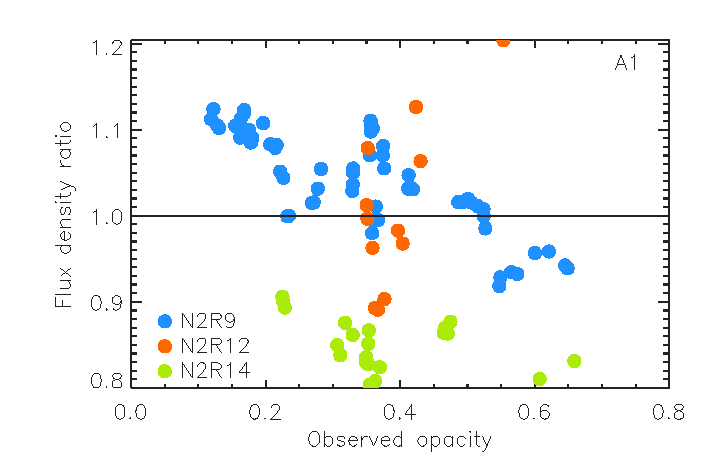
\includegraphics[clip=true,width=0.47\textwidth]{Figures/Calibration/Photocorr/plot_flux_density_ratio_MWC349_obstau_secondary_photocorr_pointing_a1.pdf}
%    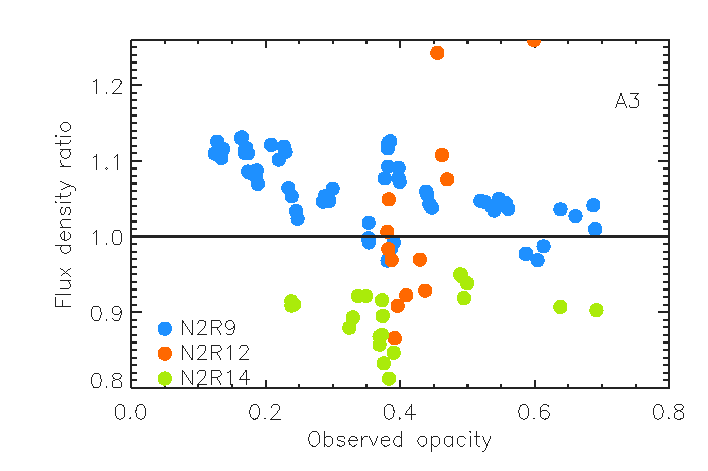
\includegraphics[clip=true,width=0.47\textwidth]{Figures/Calibration/Photocorr/plot_flux_density_ratio_MWC349_obstau_secondary_photocorr_pointing_a3.pdf}
%    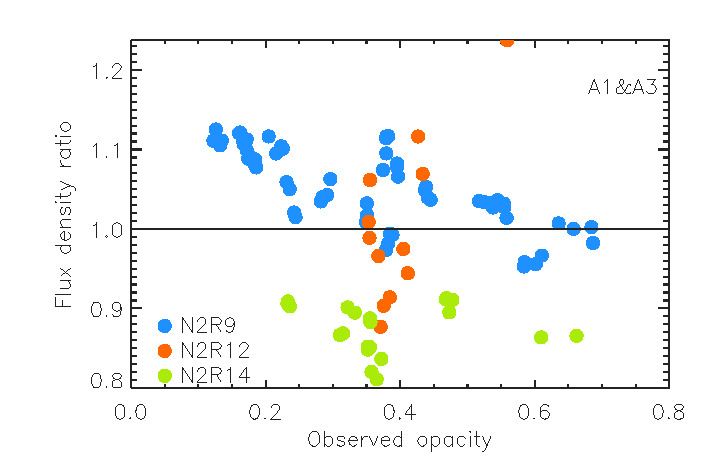
\includegraphics[clip=true,width=0.47\textwidth]{Figures/Calibration/Photocorr/plot_flux_density_ratio_MWC349_obstau_secondary_photocorr_pointing_1mm.pdf}
%    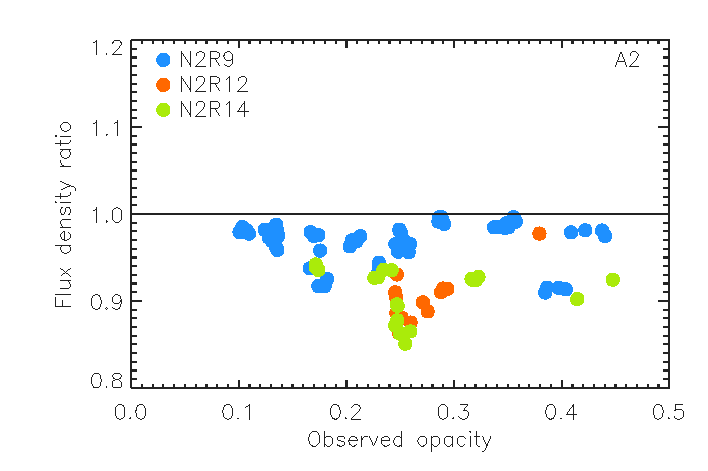
\includegraphics[clip=true,width=0.47\textwidth]{Figures/Calibration/Photocorr/plot_flux_density_ratio_MWC349_obstau_secondary_photocorr_pointing_a2.pdf}
%    \caption[MWC349 flux density stability against observed
%      opacity using pointing-based photometric correction]{Validation
%      of the calibration relying on pointing-based photometric
%      corrections.
%      Datapoints show the measured-to-modeled flux density ratio for the
%      secondary calibrator MWC349 as a fonction
%      of the measured observed opacity for array 1 (upper left), array 3
%      (upper right), 1mm array combination (lower left) and array 2 (lower
%      right). The color coding is the same as in Fig.~\ref{fig:mwc349_flux_obstau}.
%    }
%    \label{fig:mwc349_flux_obstau_photocorr_pointing}
%  \end{center}
%\end{figure}



\begin{table}[th]
\begin{center}
\begin{tabular}{|c|c|cccc|}
\hline
Runs & Arrays & $\#$Total scans   & $\#$Selected scans & Flux density bias  & Relative error \\ 
\hline\hline
 N2R9   & A1        & 64                 &  64         & 1.04               &  5.5    \\ 
        & A3        &                    &             & 1.06               &  4.5     \\ 
        & A1$\&$A3  &                    &             & 1.05               &  4.7    \\ 
        & A2        &                    &             & 0.97               &  2.4    \\ 
 \hline
 N2R12  & A1        & 13                 &  13         & 1.03               &  11.4   \\ 
        & A3        &                    &             & 1.02               &  12.0    \\ 
        & A1$\&$A3  &                    &             & 1.02               &  11.7    \\ 
        & A2        &                    &             & 0.90               &   3.2     \\
 \hline
 N2R14  & A1        & 21                 &  21         & 0.85               &  3.5    \\ 
        & A3        &                    &             & 0.90               &  4.1    \\ 
        & A1$\&$A3  &                    &             & 0.88               &  3.6    \\ 
        & A2        &                    &             & 0.91               &  3.3    \\
 \hline
combined & A1        &  98                & 98         &  1.00              &  10.0  \\ 
         & A3        &                    &            &  1.02              &  8.7   \\ 
         & A1$\&$A3  &                    &            &  1.01              &  9.2   \\ 
         & A2        &                    &            &  0.95              &  4.1   \\
\hline\hline
\end{tabular}
\caption[Beam-variation hardened calibration results using MWC349: the
practical case]{Beam-variation hardened calibration results using
  MWC349 photometry: the practical case. For the observation runs or combination of runs indicated in the first column, we report the total number of observation scans in the third column, the number of scan after the baseline selection in the fourth column, the flux density biases in the fifth, which correspond to the average measured-to-expected flux density ratios, and the relative errors given in percent in the last column, which are the $1\sigma$ errors with respect to the mean flux densities.}
\label{tab:photocorr_pointing_calib_result_mwc349}
\end{center}
\end{table}


In Fig.~\ref{fig:photocorr_pointing_secondcalib_flux_1_2_mm}, we further check the flux density stability against
the estimated beam size using other secondary calibrators.


%\begin{figure}[ht!]
%  \begin{center}
%    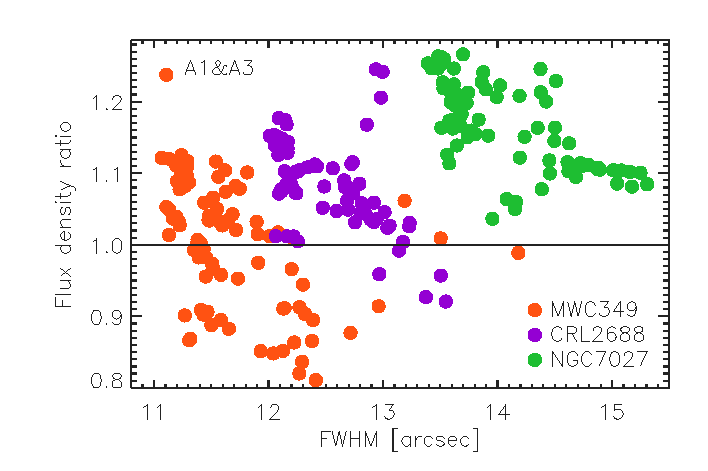
\includegraphics[clip=true,width=0.47\textwidth]{Figures/Calibration/Photocorr/plot_flux_density_ratio_3sources_FWHM_secondary_photocorr_pointing_1mm.pdf}
%    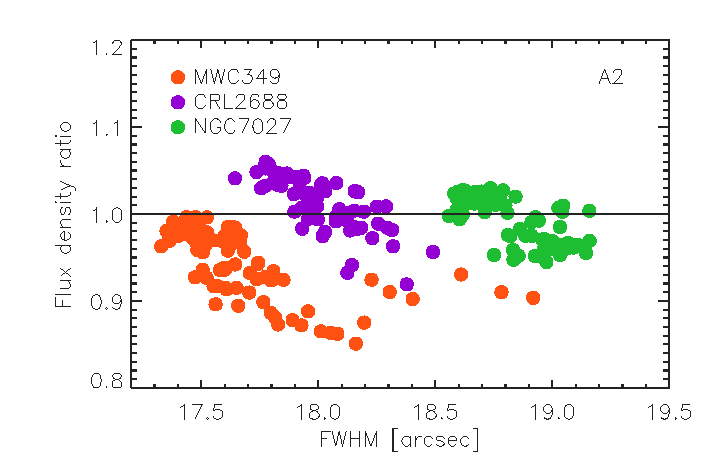
\includegraphics[clip=true,width=0.47\textwidth]{Figures/Calibration/Photocorr/plot_flux_density_ratio_3sources_FWHM_secondary_photocorr_pointing_a2.pdf}
%    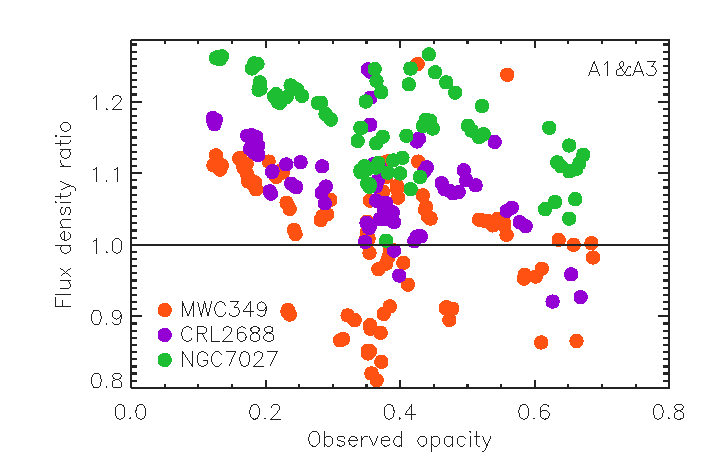
\includegraphics[clip=true,width=0.47\textwidth]{Figures/Calibration/Photocorr/plot_flux_density_ratio_3sources_obstau_secondary_photocorr_pointing_1mm.pdf}
%    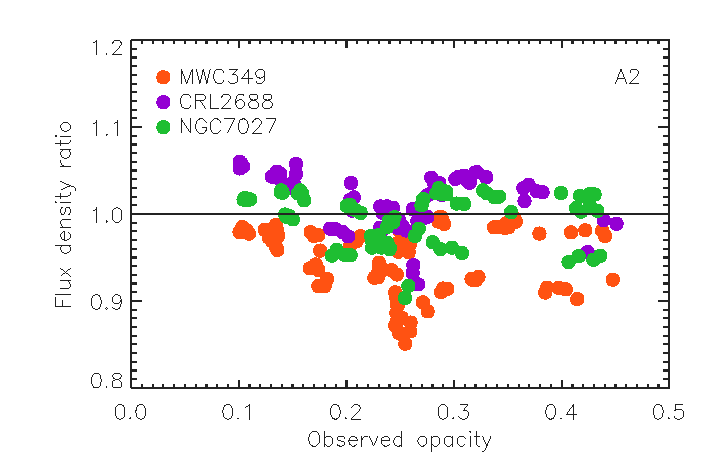
\includegraphics[clip=true,width=0.47\textwidth]{Figures/Calibration/Photocorr/plot_flux_density_ratio_3sources_obstau_secondary_photocorr_pointing_a2.pdf}
%    \caption[Flux density stability against observing conditions using
%      secondary calibrators]{Measured-to-modeled flux density ratio
%      for the three considered secondary calibrators as a function of
%      the measured FWHM (upper plots) and the observed opacity
%      (lower plots) at $1~\rm{mm}$ (left) and $2~\rm{mm}$ (right).
%      }
%    \label{fig:photocorr_pointing_secondcalib_flux_1_2_mm}
%  \end{center}
%\end{figure}
